\documentclass[11pt,letterpaper]{article}

\usepackage[T1]{fontenc}
\usepackage{lmodern}
\usepackage[margin=0.92in]{geometry}
\usepackage{amsmath,amssymb,amsthm}
\usepackage{booktabs}
\usepackage{array}
\usepackage{xcolor}
\usepackage{tikz}
\usetikzlibrary{arrows.meta,positioning,shapes.geometric,fit,backgrounds}
\usepackage{pgfplots}
\pgfplotsset{compat=1.18}
\usepackage{microtype}
\usepackage{hyperref}
\usepackage{enumitem}
\usepackage{fancyhdr}

\definecolor{cmDark}{HTML}{0B1320}
\definecolor{cmEmerald}{HTML}{059669}
\definecolor{cmCyan}{HTML}{0284C7}
\definecolor{cmGold}{HTML}{D97706}
\definecolor{cmCrimson}{HTML}{DC2626}
\definecolor{cmViolet}{HTML}{7C3AED}
\definecolor{cmSlate}{HTML}{475569}

\hypersetup{
  colorlinks=true,
  linkcolor=cmCyan,
  citecolor=cmEmerald,
  urlcolor=cmCyan,
  pdftitle={CELLULOGONIC MECHA v1.2.1: Non-Equilibrium Chemiosmotic, Elastic-Membrane, Endosymbiotic, Bioelectric, and Morphogenetic-GRN Cellular Artificial Life Laboratory with 58 Pure Lean 4 Formal Proofs},
  pdfauthor={Alexander Stephen Donahue (0thernes LLC, ORCID 0009-0006-8168-9648)}
}

\pagestyle{fancy}
\setlength{\headheight}{14pt}
\fancyhf{}
\fancyhead[L]{\footnotesize\textsc{CELLULOGONIC MECHA v1.2.1 --- Cellular Artificial Life Lab}}
\fancyhead[R]{\footnotesize\textsc{Donahue (0thernes LLC)}}
\fancyfoot[C]{\footnotesize\thepage}
\renewcommand{\headrulewidth}{0.4pt}

\newtheorem{theorem}{Theorem}
\newtheorem{proposition}[theorem]{Proposition}
\theoremstyle{remark}
\newtheorem{remark}{Remark}

\newcommand{\code}[1]{{\ttfamily\footnotesize\def\_{\textunderscore\penalty0\hskip0pt}#1}}
\emergencystretch=2.5em

\title{\vspace{-2.0em}\Large\textbf{CELLULOGONIC MECHA: A Clean-Room Non-Equilibrium Chemiosmotic, Elastic-Membrane, Endosymbiotic, Bioelectric, and Morphogenetic-GRN Cellular Artificial Life Laboratory with 58 Pure Lean~4 Formal Proofs}}

\author{%
  \textbf{Alexander Stephen Donahue}\thanks{%
    ORCID: \href{https://orcid.org/0009-0006-8168-9648}{\texttt{0009-0006-8168-9648}}.
    Affiliation: 0thernes LLC, Spokane, WA, USA.
    Email: \href{mailto:0_0@0thernes.art}{\texttt{0\_0@0thernes.art}}.
    Web: \href{https://0thernes.art}{\texttt{https://0thernes.art}}.
    Repository: \href{https://github.com/0thernes/cellulogonic-mecha}{\texttt{https://github.com/0thernes/cellulogonic-mecha}}.
    Release \texttt{v1.2.1} (\texttt{75661bb}); Software Heritage archival snapshot \texttt{swh:1:snp:383e93602d8aeda92aa413e318e8dd9848f0da56}.
    Self-funded independent research; governed by the Cosmogonic License (Non-Commercial Research \& Play).
  }\\
  \small 0thernes LLC, Spokane, WA, USA
}

\date{\vspace{-0.4em}November 21, 2026 \quad $\cdot$ \quad Technical Research Preprint \texttt{v1.2.1}}

\begin{document}
\maketitle
\thispagestyle{plain}
\vspace{-0.8em}

\begin{abstract}
We present \textbf{CELLULOGONIC MECHA \texttt{v1.2.1}}, a clean-room, zero-dependency C11 artificial-life laboratory bridging non-conservative toy simulations and intractable atomistic whole-cell models. Operating as \textbf{Build~2 (CELLULAR)} of a four-build ecosystem (\texttt{AUTOPHAGE} DNA $\to$ \texttt{Cellulogonic Mecha} Cellular $\to$ \texttt{Asmodensius} Creatures $\to$ \texttt{Asmodensius-Native} World), the engine couples eight cellular and developmental mechanisms inside an exact integer-quantum continuous $32\times 32\times 32\,\mu\mathrm{m}$ 3D fluid chamber: (i)~an 8-species, 17-reaction Chemoton with $0\,\mathrm{amu}$ mass residual, $0\,\mathrm{uq}$ First-Law energy residual, and strictly monotone Second-Law heat dissipation; (ii)~continuous 3D Stokes hydrodynamics, Hertz soft-body collisions, chemotaxis, actomyosin breathing, and stateful ATP-pumped Fr\"ohlich--Pokorn\'y $1.2\text{--}14.8\,\mathrm{GHz}$ microtubule modes (with CPUID-guarded \texttt{RDSEED}); (iii)~discrete Canham--Helfrich elastic bilayers governing lysis, symmetric fission ($Q \le \tfrac{1}{2}$), and asymmetric budding ($\tfrac{1}{2} < Q < 1$); (iv)~Mitchell chemiosmosis with evolvable c-rings across four planetary solvents; (v)~Nick Lane's $1/R$ ceiling shattered by nested primary and secondary endosymbiosis; (vi)~Michael Levin's bioelectric gap-junction morphogenesis and cancer policing; (vii)~tardigrade TDP/CAHS bioglass anhydrobiosis; and (viii)~zero-blueprint 3D embryogenesis combining Z-stratified \texttt{Wnt/BMP/Shh} GPS, conditional GRNs, Steinberg cadherin sorting, apical constriction, Netrin/Slit axon guidance with Hebbian pruning, Hippo/eutelic growth arrest, and ATP-coupled (\texttt{RXN\_R8}) CPG steering.

Every core invariant is machine-checked across \textbf{58 pure Lean~4 (\texttt{v4.35.0}) theorems} (\texttt{T01}--\texttt{T58}, 8 modules, 1,438 lines, zero Mathlib, zero \texttt{sorryAx}, zero custom axioms, zero warnings, strictly within \texttt{[propext, Classical.choice, Quot.sound]}), including an elementary sextic proof of the \textbf{Global Minimax Theorem of Vesicle Division} (\texttt{T16}). Across Win64 PE64 (\texttt{clang 23.1.0}) and Ubuntu Linux ELF64 (\texttt{gcc 13.3.0}), both 256-bit AVX2 ($31.181\,\mathrm{M\,rxns/s}$ Linux, $30.281\,\mathrm{M\,rxns/s}$ Win64) and scalar kernels agree to \textbf{0-bit SHA-256 diff} (\texttt{f20e16ec\ldots 4f26e918}) and pass \textbf{24/24 falsification gates} catching \textbf{8/8 planted mutants}. From zero living cells, the soup condenses 1,715 vesicles peaking at 607 cells ($\mathrm{COVI} = 90.26$, Stage~6); from 8 identical-DNA blastomeres, 3D embryogenesis self-organizes 58 differentiated cells (78.1\% homotypic sorting, 80 guided axons, 39 pruned, 398 CPG pulses, 0 drift). On locked paired seeds ($N = 24$), all four pre-registered hypotheses achieve $p_{\mathrm{Holm}} \le 0.00080$.
\end{abstract}

\noindent\textbf{Keywords:} artificial life, chemoton, autopoiesis, Canham--Helfrich vesicles, chemiosmosis, endosymbiosis, bioelectricity, morphogenesis, gene regulatory networks, Lean~4 formal verification, deterministic SIMD simulation.

% =====================================================================
\section{Introduction and Four-Build Clean-Room Architecture}
\label{sec:intro}
% =====================================================================

Life on Earth is fundamentally cellular. Prior to nervous systems, macroscopic anatomy, or symbolic cognition, living matter solved nanoscale autopoiesis~\cite{varela1974,ganti1975}, chemiosmotic energy transduction~\cite{mitchell1961}, elastic bilayer morphogenesis~\cite{canham1970,helfrich1973}, symbiogenetic compartmentalization~\cite{margulis1967,lane2010}, and multicellular bioelectric and morphogenetic coordination~\cite{levin2022,wolpert1969,steinberg1963}. Yet computational Artificial Life (ALife) faces a methodological chasm:
\begin{enumerate}[leftmargin=1.8em, itemsep=2pt]
  \item \textbf{Non-Conservative Abstract Sandboxes:} Cellular automata, neural CA, and particle-life engines generate compelling visual motifs but routinely omit atomic mass conservation, First- and Second-Law thermodynamic closure, endergonic biosynthetic coupling, osmotic membrane mechanics, and $1/R$ bioenergetic scaling walls. Without conservation closure, evolutionary trajectories rapidly saturate or exploit simulator artifacts~\cite{bedau1998,taylor2016}.
  \item \textbf{Intractable Atomistic Whole-Cell Models:} Landmark whole-cell simulations---including the Stanford \emph{Mycoplasma genitalium} model~\cite{karr2012} and the Illinois 4D \emph{JCVI-syn3A} minimal cell~\cite{hutchison2016,breuer2019,pelletier2021,thornburg2022}---achieve molecular fidelity for a single bacterium at the cost of hours per cell cycle, making thousand-cell eukaryotic populations or eutelic micro-metazoans~\cite{szigeti2014} intractable on consumer workstations.
\end{enumerate}

\textbf{CELLULOGONIC MECHA \texttt{v1.2.1}} occupies the rigorous middle ground: an \emph{exact discrete biophysical laboratory} that strips away explicit solvent atomic coordinates while preserving exact integer atomic mass conservation, exact First- and Second-Law thermodynamic closure, exact Canham--Helfrich geometric thresholds, developmental Gene Regulatory Networks, and nested compartmentalized heredity at $30\text{--}31\,\mathrm{M}$ conserved reactions per second in continuous 3D off-lattice space on a single consumer CPU.

To eliminate false-positive emergence claims, the engine enforces four Clean-Slate invariants inherited from Build~4 (\texttt{Asmodensius-Native}):
\begin{itemize}[leftmargin=1.6em, itemsep=2pt]
  \item \textbf{\texttt{P2} (Exact Conservation \& Thermodynamic Arrow):} Atomic mass (\texttt{int64\_t} amu) and First-Law energy (\texttt{int64\_t} uq) close to identically $0$ residual every tick; the radiated heat sink is strictly non-decreasing (\texttt{second\_law\_violations == 0}).
  \item \textbf{\texttt{P4} (Domain-Isolated Stochasticity \& Authenticated Snapshots):} Deterministic runs draw from five domain-isolated counter-based \texttt{Philox4x32-10} streams (\texttt{WORLD\_EXOG}, \texttt{ABIOGENESIS}, \texttt{CELL\_MUT}, \texttt{MITOSIS\_PART}, \texttt{PHAGO\_HGT}); binary \texttt{.cmbin} snapshots append a NIST FIPS~180-4 SHA-256 integrity trailer verified prior to deserialization; feral mode (\texttt{seed=0}) invokes CPUID-guarded Intel \texttt{RDSEED} hardware thermal entropy.
  \item \textbf{\texttt{P9} (Strict Observer Independence):} Telemetry computation, apex specimen inspection, and live 60~FPS WebGL2 Observatory JSON export accept strictly \texttt{const CellWorld*} and produce 0-bit SHA-256 divergence from headless execution.
  \item \textbf{\texttt{P10} / \texttt{HW02} (Zero Post-Warmup Allocations):} All spatial grids, diffusion accumulators, and scratch pools allocate once inside \texttt{cellulogonic\_create()}; \texttt{post\_warmup\_allocs == 0} across stepping.
\end{itemize}

Figure~\ref{fig:arch} illustrates the 4-build ecosystem integration and the eight coupled cellular subsystems inside \texttt{CELLULOGONIC MECHA}. Through its flat C11 ABI (\code{include/cellulogonic\_abi.h}), Build~2 connects downward to Build~1 (\texttt{AUTOPHAGE}) via \code{cellulogonic\_ingest\_autophage\_genome()} (SHA-256 folding of 256-byte dual-strand organisms into 128-byte cellular operons) and upward to Build~3 (\texttt{Asmodensius}) via \code{cellulogonic\_project\_asmodensius\_112()} (clamped $[0,1]^{112}$ trait projection).

\begin{figure}[ht]
\centering
\resizebox{\textwidth}{!}{%
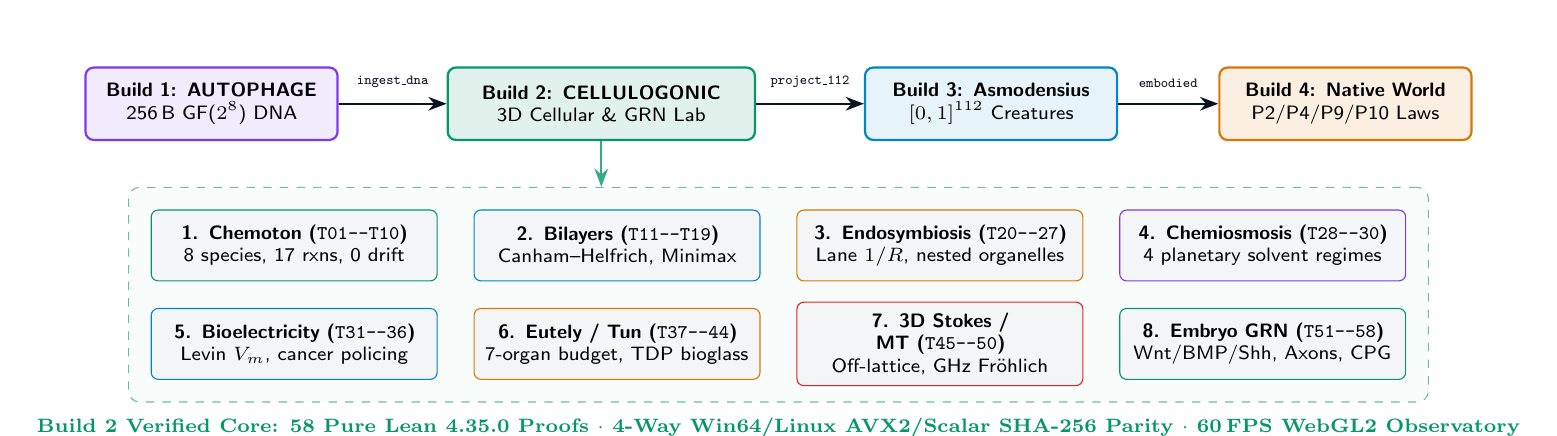
\begin{tikzpicture}[
  font=\scriptsize\sffamily,
  >=Stealth,
  box/.style={draw, rounded corners=3pt, thick, align=center, inner sep=5pt, minimum height=0.92cm},
  sub/.style={draw=cmSlate, rounded corners=2.5pt, fill=cmSlate!6, align=center, inner sep=4pt, text width=3.35cm, minimum height=0.90cm}
]
  % Top 4-build pipeline with generous horizontal gap for edge labels
  \node[box, draw=cmViolet, fill=cmViolet!10, text width=2.85cm] (b1) at (0,0) {\textbf{Build 1: AUTOPHAGE}\\256\,B GF($2^8$) DNA};
  \node[box, draw=cmEmerald, fill=cmEmerald!12, text width=3.55cm] (b2) at (4.95,0) {\textbf{Build 2: CELLULOGONIC}\\3D Cellular \& GRN Lab};
  \node[box, draw=cmCyan, fill=cmCyan!10, text width=2.85cm] (b3) at (9.90,0) {\textbf{Build 3: Asmodensius}\\$[0,1]^{112}$ Creatures};
  \node[box, draw=cmGold, fill=cmGold!12, text width=2.85cm] (b4) at (14.40,0) {\textbf{Build 4: Native World}\\P2/P4/P9/P10 Laws};

  \draw[->, thick, cmDark] (b1) -- node[above=2pt, font=\tiny\ttfamily] {ingest\_dna} (b2);
  \draw[->, thick, cmDark] (b2) -- node[above=2pt, font=\tiny\ttfamily] {project\_112} (b3);
  \draw[->, thick, cmDark] (b3) -- node[above=2pt, font=\tiny\ttfamily] {embodied} (b4);

  % 8 coupled subsystems grid below Build 2 with clean vertical separation
  \node[sub, draw=cmEmerald] (s1) at (1.05,-1.80) {\textbf{1. Chemoton (\texttt{T01--T10})}\\8 species, 17 rxns, 0 drift};
  \node[sub, draw=cmCyan]    (s2) at (5.15,-1.80) {\textbf{2. Bilayers (\texttt{T11--T19})}\\Canham--Helfrich, Minimax};
  \node[sub, draw=cmGold]    (s3) at (9.25,-1.80) {\textbf{3. Endosymbiosis (\texttt{T20--27})}\\Lane $1/R$, nested organelles};
  \node[sub, draw=cmViolet]  (s4) at (13.35,-1.80) {\textbf{4. Chemiosmosis (\texttt{T28--30})}\\4 planetary solvent regimes};

  \node[sub, draw=cmCyan]    (s5) at (1.05,-3.05) {\textbf{5. Bioelectricity (\texttt{T31--36})}\\Levin $V_m$, cancer policing};
  \node[sub, draw=cmGold]    (s6) at (5.15,-3.05) {\textbf{6. Eutely / Tun (\texttt{T37--44})}\\7-organ budget, TDP bioglass};
  \node[sub, draw=cmCrimson] (s7) at (9.25,-3.05) {\textbf{7. 3D Stokes / MT (\texttt{T45--50})}\\Off-lattice, GHz Fr\"ohlich};
  \node[sub, draw=cmEmerald] (s8) at (13.35,-3.05) {\textbf{8. Embryo GRN (\texttt{T51--58})}\\Wnt/BMP/Shh, Axons, CPG};

  \begin{scope}[on background layer]
    \node[draw=cmEmerald!60, dashed, rounded corners=4pt, fill=cmEmerald!3, fit=(s1)(s4)(s5)(s8), inner sep=8pt, label={[font=\scriptsize\bfseries\color{cmEmerald}, yshift=-2pt]below:Build 2 Verified Core: 58 Pure Lean~4.35.0 Proofs $\cdot$ 4-Way Win64/Linux AVX2/Scalar SHA-256 Parity $\cdot$ 60\,FPS WebGL2 Observatory}] (core) {};
  \end{scope}

  \draw[->, thick, cmEmerald!80] (b2.south) -- (b2.south |- core.north);
\end{tikzpicture}%
}
\caption{Four-build artificial-life ecosystem integration and the eight coupled cellular/developmental biophysical subsystems verified inside \texttt{CELLULOGONIC MECHA v1.2.1}.}
\label{fig:arch}
\end{figure}

% =====================================================================
\section{Theorem I: Exact Integer-Quantum Chemoton Stoichiometry and Thermodynamics}
\label{sec:chemoton}
% =====================================================================

Following G\'anti's Chemoton~\cite{ganti1975,ganti2003}, Rosen's $(M,R)$-systems~\cite{rosen1958}, and Schnakenberg's network thermodynamics~\cite{schnakenberg1976}, every spatial voxel and every cellular or organelle compartment maintains exact non-negative integer counts $\mathbf{n} \in \mathbb{Z}_{\ge 0}^8$ over eight conserved molecular species (substrate, oxidant, reduced cofactor, ATP, amphiphilic lipid, folded catalytic polypeptide, informational template polymer, and exhaust waste):
\begin{equation}
  \begin{aligned}
    \mathcal{S} &= (\mathrm{S}, \mathrm{X}, \mathrm{M}, \mathrm{E}, \mathrm{L}, \mathrm{P}, \mathrm{T}, \mathrm{W}), \\
    \mathbf{w}  &= (4, 2, 6, 4, 8, 12, 16, 2)\,\mathrm{amu}, \qquad
    \boldsymbol{\mu} = (48, 36, 80, 40, 104, 156, 212, 6)\,\mathrm{uq}.
  \end{aligned}
\end{equation}

\begin{theorem}[Chemoton Stoichiometry \& Thermodynamics; {\normalfont\ttfamily\footnotesize StoichiometryThermo.lean}, {\normalfont\ttfamily T01--T10}]
\label{thm:chemoton}
Let $\mathcal{R} = \{\mathrm{R1}, \dots, \mathrm{R14b}\}$ be the 17 cellular reactions with stoichiometric vectors $\boldsymbol{\nu}_r \in \mathbb{Z}^8$, proton-motive quanta $\Delta p_r \in \mathbb{Z}$, external energy inflow $E_r^{\mathrm{in}} \ge 0$, and irreversible heat dissipation $q_r \in \mathbb{Z}$. Then:
\begin{enumerate}[leftmargin=1.8em, itemsep=1.5pt]
  \item \textbf{Exact Atomic Mass Conservation} (\textup{\texttt{T01, T07, T10}}): $\forall r \in \mathcal{R}$, $\mathbf{w}^\top \boldsymbol{\nu}_r = 0$. Arbitrary reaction multiplicities $k \ge 0$, binary fissions, and phagocytic engulfments conserve total world atomic mass identically ($\Delta M_{\mathrm{world}} = 0$).
  \item \textbf{Exact First-Law Energy Balance} (\textup{\texttt{T02, T08}}): $\forall r \in \mathcal{R}$, $\boldsymbol{\mu}^\top \boldsymbol{\nu}_r + \Delta p_r \cdot e_{\mathrm{pmf}} + q_r = E_r^{\mathrm{in}}$, closing the global ledger $E_{\mathrm{chem}} + E_{\mathrm{pmf}} + E_{\mathrm{heat,local}} + E_{\mathrm{heat,sink}} - E_{\mathrm{inflow}} = E_0$ to identically $0\,\mathrm{uq}$.
  \item \textbf{Strict Second-Law Dissipation \& No Perpetual Motion} (\textup{\texttt{T03, T06, T09}}): $\forall r \in \mathcal{R}$, $q_r > 0$. Any non-empty closed thermodynamic trajectory $(r_1, \dots, r_m)$ returning all chemical and PMF states to their origin ($\sum \Delta G = 0$) satisfies $\sum_{j=1}^m q_{r_j} > 0$ and strictly requires equal external free-energy inflow $\sum_{j=1}^m E_{r_j}^{\mathrm{in}} = \sum_{j=1}^m q_{r_j} > 0$.
  \item \textbf{Mandatory ATP Coupling \& $4\times$ Respiratory Yield} (\textup{\texttt{T04, T05}}): Uncoupled biosynthesis of lipids ($2\mathrm{S} \to \mathrm{L}$, $\Delta G = +8$), polypeptides ($3\mathrm{S} \to \mathrm{P}$, $\Delta G = +12$), and templates ($4\mathrm{S} \to \mathrm{T}$, $\Delta G = +20$) is strictly endergonic and gated on ATP hydrolysis ($\mathrm{E} \to 2\mathrm{W}$, $\Delta G = -28$). Oxidative chemiosmotic respiration ($\mathrm{R1} + \mathrm{R2} + 2\cdot\mathrm{R3}$) yields $2\,\mathrm{E}$ per $1\,\mathrm{S}$, whereas anaerobic fermentation ($\mathrm{R4}: 2\mathrm{S} \to \mathrm{E} + 2\mathrm{W}$) yields $1\,\mathrm{E}$ per $2\,\mathrm{S}$---an exact $4\times$ yield advantage.
\end{enumerate}
\end{theorem}

% =====================================================================
\section{Theorem II: Discrete Canham--Helfrich Vesicles and the Global Minimax Theorem of Vesicle Division}
\label{sec:vesicles}
% =====================================================================

A closed lipid vesicle with membrane area $A \propto L$ and internal osmolyte volume $V$ is governed by its dimensionless reduced volume $\nu = 6\sqrt{\pi}\,V / A^{3/2}$, whose cleared-denominator square $Q(V, L) = C_0 V^2 / L^3$ (with exact integer scale $C_0 = 100$) determines Canham--Helfrich elastic bending stability and osmotic lysis~\cite{canham1970,helfrich1973,zhu2009,svetina2009}.

\begin{theorem}[Global Minimax Theorem of Vesicle Division; {\normalfont\ttfamily\footnotesize MembraneGeometry.lean}, {\normalfont\ttfamily T11--T19}]
\label{thm:minimax}
For integer vesicle states $(V, L) \in \mathbb{N}_+^2$:
\begin{enumerate}[leftmargin=1.8em, itemsep=1.5pt]
  \item \textbf{Symmetric Binary Fission Exact Threshold} (\textup{\texttt{T11--T13}}): Halving $(2v, 2l) \mapsto (v, l)$ strictly doubles $Q$. Two equal intact spherical daughters ($C_0 v^2 \le l^3$) exist \emph{if and only if} $Q_{\mathrm{parent}} \le \tfrac{1}{2}$ ($2 C_0 V^2 \le L^3$). Every intact vesicle in the swollen interphase window $\tfrac{1}{2} < Q \le 1$ is strictly blocked from symmetric fission.
  \item \textbf{Proportional Split Suboptimality \& Exosome Escape} (\textup{\texttt{T14, T15}}): Any split preserving equal area-to-volume ratios ($V_1/L_1 = V_2/L_2 = V/L$) forces $\max(Q_1, Q_2) \ge 2 Q_{\mathrm{parent}}$. By contrast, at $(V = 47, L = 72)$ where $Q = 0.592 > \tfrac{1}{2}$ forbids symmetric division, strain-matched asymmetric budding into $(6, 16) + (41, 56)$ yields two strictly intact spheres ($Q_1 = 0.879 \le 1$, $Q_2 = 0.957 \le 1$).
  \item \textbf{Exact Sextic Minimax Identity} (\textup{\texttt{T16}}): Writing daughter volumes $V_1 = x^3, V_2 = y^3$ ($x, y > 0$) and strain-matched minimal spherical areas $L_1 = x^2, L_2 = y^2$,
  \begin{equation}
    2(x^3 + y^3)^2 - (x^2 + y^2)^3 = (x - y)^2 \bigl(x^4 + 2x^3 y + 2x y^3 + y^4\bigr) \ge 0,
    \label{eq:sextic}
  \end{equation}
  with strict inequality whenever $x \neq y$ and equality \emph{if and only if} $x = y$. Hence symmetric binary fission ($x = y$) is the unique global maximum of membrane-area demand among all binary vesicle splits, proving from elementary algebra why swollen vesicles ($\tfrac{1}{2} < Q < 1$) shed exosomes or asymmetric buds.
\end{enumerate}
\end{theorem}

Figure~\ref{fig:minimax} plots the exact feasible parent reduced-volume ceiling $Q_{\max}(f) = \bigl(f^3 + (1-f)^3\bigr)^2 / \bigl(f^2 + (1-f)^2\bigr)^3$ against linear daughter radius fraction $f = x / (x+y)$, illustrating why $f = 0.5$ is the unique global bottleneck at $Q_{\max}(0.5) = 0.5$ while asymmetric budding unlocks the entire swollen interphase window $\tfrac{1}{2} < Q < 1$.

\begin{figure}[ht]
\centering
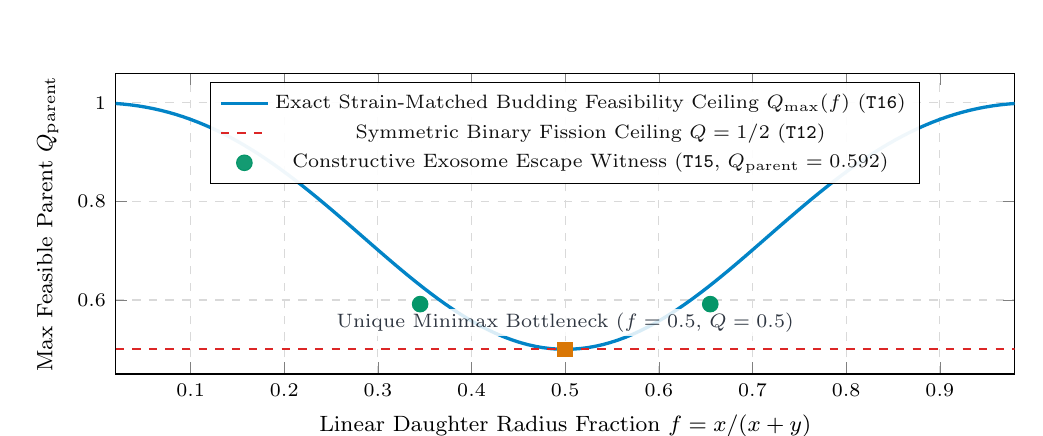
\begin{tikzpicture}
\begin{axis}[
  width=13.0cm, height=5.4cm,
  xlabel={Linear Daughter Radius Fraction $f = x / (x + y)$},
  ylabel={Max Feasible Parent $Q_{\mathrm{parent}}$},
  xmin=0.02, xmax=0.98,
  ymin=0.45, ymax=1.06,
  grid=major,
  grid style={dashed, gray!30},
  legend style={at={(0.5,0.97)}, anchor=north, font=\scriptsize, fill=white, fill opacity=0.94},
  label style={font=\footnotesize},
  tick label style={font=\scriptsize}
]
  \addplot[color=cmCyan, very thick, domain=0.02:0.98, samples=121]
    { ((x^3 + (1-x)^3)^2) / ((x^2 + (1-x)^2)^3) };
  \addlegendentry{Exact Strain-Matched Budding Feasibility Ceiling $Q_{\max}(f)$ (\texttt{T16})}

  \addplot[color=cmCrimson, thick, dashed, domain=0.02:0.98, samples=2] {0.5};
  \addlegendentry{Symmetric Binary Fission Ceiling $Q = 1/2$ (\texttt{T12})}

  \addplot[only marks, mark=*, mark size=2.8pt, color=cmEmerald] coordinates {(0.3451, 0.5917) (0.6549, 0.5917)};
  \addlegendentry{Constructive Exosome Escape Witness (\texttt{T15}, $Q_{\mathrm{parent}} = 0.592$)}

  \addplot[only marks, mark=square*, mark size=2.6pt, color=cmGold] coordinates {(0.5, 0.5)};
  \node[font=\scriptsize, anchor=south, color=cmDark, fill=white, fill opacity=0.85, inner sep=1.5pt] at (axis cs:0.5,0.525) {Unique Minimax Bottleneck ($f=0.5$, $Q=0.5$)};
\end{axis}
\end{tikzpicture}
\caption{Geometric consequence of the sextic factorization~\eqref{eq:sextic} (\texttt{T16}). Symmetric halving ($f = 0.5$) minimizes feasible parent reduced volume at $Q_{\max}(0.5) = \tfrac{1}{2}$, whereas strain-matched asymmetric budding ($f \neq 0.5$) strictly raises $Q_{\max}(f) \to 1$, enabling the constructive exosome witness \texttt{T15} ($(47,72) \to (6,16) + (41,56)$, $Q_{\mathrm{parent}} = 0.592$).}
\label{fig:minimax}
\end{figure}

% =====================================================================
\section{Theorems III--VII: Endosymbiosis, Chemiosmosis, Bioelectricity, Eutely, Cytoskeleton, and Developmental GRNs}
\label{sec:theorems}
% =====================================================================

Beyond Chemoton closure and elastic bilayer geometry, five additional Lean~4 modules formalize the scaling, planetary, multicellular, nanomechanical, and developmental laws of the engine (consolidated in Table~\ref{tab:lean}).

\begin{itemize}[leftmargin=1.6em, itemsep=2pt]
  \item \textbf{Theorem III --- Lane's $1/R$ Ceiling \& Endosymbiosis} (\code{Bioenergetics\allowbreak Endosymbiosis.lean}, \texttt{T20}--\texttt{T27}): With outer area $A(R) = 3R^2$ and volume $V(R) = R^3$, prokaryotic surface power $3 c_A R^2$ exceeds volumetric maintenance $c_V R^3$ \emph{if and only if} $c_V R < 3 c_A$ (\texttt{T20}), while specific power density $3 c_A / R$ strictly declines (\texttt{T21})~\cite{lane2010}. Internalizing $K$ respiratory endosymbionts of radius $r < R$ amplifies respiratory area per volume by $R/r > 1$ (\texttt{T23}), permitting $P_{\mathrm{euk}} = 3 c_A R^2 + 3 K c_{\mathrm{endo}} r^2 > c_V R^3$ for arbitrarily large host radius $R$ (\texttt{T22})~\cite{margulis1967}, with depth-2 secondary chimeras adding strictly positive power (\texttt{T24}). Uneven mitotic partitioning of $c = c_1 + c_2$ cooperative and $s = s_1 + s_2$ selfish organelles ($c_1 s_2 \neq c_2 s_1$) guarantees one daughter strictly improves cooperative fraction while the other worsens, enabling host-level purifying selection (\texttt{T26}), while Endosymbiotic Gene Transfer (EGT) cuts replication cost by $(K - 1)g > 0$ (\texttt{T27}).
  \item \textbf{Theorem IV --- Solvent c-Rings, Levin Bioelectricity \& Anti-Gaming} (\code{Chemiosmosis\allowbreak Autopoiesis.lean}, \texttt{T28}--\texttt{T36}): Phosphorylation ($\Delta G_{\mathrm{ATP}} = 28\,\mathrm{uq}$) requires $n_H \cdot e_{\mathrm{pmf}} \ge 28$, certifying exact planetary c-ring stoichiometry floors: Terran $\mathrm{H}_2\mathrm{O}$ and hydrothermal GDGT monolayers ($e_{\mathrm{pmf}} = 10$, $n_H \ge 3$, \texttt{T28})~\cite{caforio2017}, Venusian concentrated $\mathrm{H}_2\mathrm{SO}_4$ ($e_{\mathrm{pmf}} = 15$, $n_H \ge 2$, \texttt{T29})~\cite{seager2023,seager2024}, and Titan cryogenic azotosomes ($e_{\mathrm{pmf}} = 7$, $n_H \ge 4$, \texttt{T30})~\cite{stevenson2015}. Passive gap-junction coupling satisfies $g_{ij}(V_i - V_j)^2 \ge 0$ (\texttt{T31}), conserves charge, contracts voltage variance (\texttt{T33}), and monotonically dissipates Dirichlet energy (\texttt{T32}), proving sustained bioelectric prepatterns strictly require active ATP ion pumping~\cite{levin2022}. Dead lipid crystals and uncatalyzed white noise score identically $0$ on gated $\mathrm{COVI}$ (\texttt{T34}, \texttt{T35}), while Markov-blanket selectivity separates internal dynamics with exact mass conservation (\texttt{T36})~\cite{krakauer2020,hoshika2019}.
  \item \textbf{Theorem V --- 3D Hollow-Tube Geometry, Eutelic 7-Organ Budget \& Bioglass} (\code{Eutelic\allowbreak Organogenesis.lean}, \texttt{T37}--\texttt{T44}): Enclosing a non-degenerate 3D lumen requires $\ge 3 L_{\mathrm{rings}}$ epithelial cells (\texttt{T37}); summing mandatory 7-organ minima proves any discrete metazoan needs $\ge 355$ cells (with a constructive 800-cell witness, \texttt{T38})~\cite{szigeti2014}, compressible below 500 only via syncytial/myoepithelial fusion (\texttt{T39}). Hydrostatic incompressibility ($A_1 L_1 = A_2 L_2 > 0$) proves circumferential contraction forces axial elongation (\texttt{T40}); eutely grows biomass via hypertrophy at fixed cell count (\texttt{T41}); tardigrade TDP/CAHS vitrification ($D_{\mathrm{glass}} \ge 10$) suppresses decay while conserving mass across desiccation/rehydration (\texttt{T42})~\cite{boothby2017,hashimoto2016}; protonephridial flame-cell balance prevents osmotic swelling (\texttt{T43}); and 5-tier DNA-to-organism mass conservation holds identically (\texttt{T44}).
  \item \textbf{Theorem VI --- 3D Cytoskeletal Nanomechanics} (\code{Cytoskeleton\allowbreak Nanomechanics.lean}, \texttt{T45}--\texttt{T50}): Overdamped Stokes drag dissipates kinetic power non-negatively (\texttt{T45}); pairwise 3D Hertz collisions conserve linear momentum (\texttt{T46}); prolate cytokinetic elongation strictly increases surface area at fixed volume (\texttt{T47}); Fr\"ohlich--Pokorn\'y GHz microtubule coherence strictly requires metabolic ATP pumping above thermal damping (\texttt{T48})~\cite{frohlich1968,pokorny2004} with inverse-length frequency scaling (\texttt{T49})~\cite{sahu2013}; and actomyosin pulsatile work is strictly bounded by ATP hydrolysis energy (\texttt{T50}).
  \item \textbf{Theorem VII --- Developmental Morphogenetic GRNs} (\code{Morphogenetic\allowbreak GRN.lean}, \texttt{T51}--\texttt{T58}): Wolpert French-Flag morphogen thresholds partition $[0, \infty)$ completely into \texttt{Wnt/BMP/Shh} fates (\texttt{T51})~\cite{wolpert1969}; Steinberg differential cadherin adhesion strictly lowers interfacial energy under homotypic sorting (\texttt{T52})~\cite{steinberg1963}; apical actomyosin ring constriction increases epithelial wedge curvature monotonically (\texttt{T53}); binary eutelic countdowns strictly bound descendants at $2^k$ ($2^9 = 512$, $2^{10} = 1024$, \texttt{T54}); Hippo compression arrests mitosis above crowding threshold (\texttt{T55}); Hebbian activity updating strengthens active axons and prunes silent axons (\texttt{T56}); CPG pacemakers remain bounded under sensorimotor steering (\texttt{T57})~\cite{marder2001}; and structural induction over arbitrary \code{List MorphStep} trajectories proves developmental signaling, sorting, wiring, and ATP-coupled CPG propulsion introduce identically $0\,\mathrm{amu}$ mass drift and $0\,\mathrm{uq}$ energy drift (\texttt{T58}).
\end{itemize}

\begin{table}[ht]
\centering
\caption{Pure Lean~4 (\texttt{v4.35.0}, zero Mathlib) formal verification ledger (\code{results/lean4-audit.txt}). All 58 theorems compile with zero warnings, zero \texttt{sorryAx}, and zero custom axioms, strictly within \texttt{[propext, Classical.choice, Quot.sound]} (5 zero-axiom constructive theorems).}
\label{tab:lean}
\footnotesize
\setlength{\tabcolsep}{3.5pt}
\begin{tabular}{@{} l l c r >{\raggedright\arraybackslash}p{6.2cm} @{}}
\toprule
\textbf{Group} & \textbf{Lean~4 Module} & \textbf{Theorems} & \textbf{Lines} & \textbf{Machine-Checked Invariants} \\
\midrule
I   & \code{StoichiometryThermo.lean}       & \texttt{T01}--\texttt{T10} & 310 & Exact mass ($0\,\mathrm{amu}$), 1st-Law ($0\,\mathrm{uq}$), 2nd-Law $q_r>0$, ATP coupling, $4\times$ respiration, no perpetual cycles \\
II  & \code{MembraneGeometry.lean}          & \texttt{T11}--\texttt{T19} & 243 & $Q \le 1/2$ fission iff, exosome escape \texttt{T15}, sextic \textbf{Global Minimax Theorem} \texttt{T16}, osmotic lysis \\
III & \code{BioenergeticsEndosymbiosis.lean}& \texttt{T20}--\texttt{T27} & 153 & Lane $1/R$ ceiling, $O(1)$ endosymbiotic liberation, $R/r$ amplification, heteroplasmy purifying selection, EGT \\
IV  & \code{ChemiosmosisAutopoiesis.lean}   & \texttt{T28}--\texttt{T36} & 127 & Terran/Venus/Titan c-ring floors, Levin Dirichlet dissipation, crystal/noise $\mathrm{COVI}=0$, Markov blanket \\
V   & \code{EutelicOrganogenesis.lean}      & \texttt{T37}--\texttt{T44} & 165 & 3D tube lumen $\ge 3L$, 7-organ $\ge 355$ budget, syncytial compression, hydrostatic skeleton, TDP bioglass \\
VI  & \code{CytoskeletonNanomechanics.lean} & \texttt{T45}--\texttt{T50} & 114 & Stokes dissipation, Hertz momentum, prolate area excess, Fr\"ohlich GHz pumping, ATP work bound \\
VII & \code{MorphogeneticGRN.lean}          & \texttt{T51}--\texttt{T58} & 239 & Wolpert GPS, Steinberg sorting, apical wedge, eutelic $2^k$, Hippo arrest, Hebbian pruning, CPG, \texttt{List MorphStep} 0-drift \\
--- & \code{CellulogonicProofs.lean}        & Audit Entry                &  87 & Master import \& \texttt{\#print axioms} kernel audit over all 58 theorems \\
\midrule
\textbf{Total} & \textbf{8 Pure Lean~4 Modules} & \textbf{58 / 58} & \textbf{1,438} & \textbf{0 \texttt{sorryAx} $\cdot$ 0 custom axioms $\cdot$ 0 warnings (CI \texttt{\#44894602931})} \\
\bottomrule
\end{tabular}
\end{table}

% =====================================================================
\section{Computational Architecture, Anti-Fraud Hardening, and 4-Way Bit-Exact Parity}
\label{sec:arch}
% =====================================================================

CELLULOGONIC MECHA compiles with zero third-party runtime dependencies on Windows~11 PE64 (\texttt{clang 23.1.0 + lld}) and Ubuntu Linux ELF64 (\texttt{gcc 13.3.0}). Spatial diffusion executes via either a 256-bit AVX2 vector kernel (\texttt{v4i64}, exact signed truncation-toward-zero bias) or a portable scalar C11 reference oracle. Release \texttt{v1.2.1} incorporates comprehensive anti-fraud and security hardening: cryptographic SHA-256 trailers and strict cell/bond/axon bounds verification on \texttt{.cmbin} snapshots; FIFO queue deadlock elimination, timeouts, source-exposure blocking, and loopback guards in \code{web/server.mjs}; full 13-vector independent restraint parity eliminating 5 prior dead-zones; CPUID-guarded \texttt{RDSEED}/\texttt{RDRAND}; 3D Z-stratified morphogens; exact \texttt{RXN\_R8} ATP hydrolysis coupling for CPG motor pulses; a stateful Fr\"ohlich GHz relaxation ODE; catalysis-gated LZ77 Assembly Index~\cite{sharma2023}; linear-probing lineage hashing; and clamped $[0,1]^{112}$ phenotype projection.

Table~\ref{tab:parity} reports the 4-way cross-OS, cross-compiler, cross-ISA benchmark over 300 epochs in a $32\times 32\times 32\,\mu\mathrm{m}$ chamber (35,792 cell steps, 667,512 exact reactions, seed \texttt{5000}, measured on Intel Core Ultra~9 275HX). All four executions agree to \textbf{0-bit SHA-256 diff} with identically $0\,\mathrm{amu}$ mass drift, $0\,\mathrm{uq}$ energy drift, $0$ Second-Law violations, and $0$ post-warmup heap allocations.

\begin{table}[ht]
\centering
\caption{Four-way cross-OS, cross-compiler, and cross-ISA bit-exact SHA-256 verification (300 epochs, 35,792 cell steps, 667,512 reactions, seed \texttt{5000}; full 64-hex digest \code{f20e16ece7f747b887aaf7643562cee4\allowbreak 85cf6216c3bb843edfba28004f26e918}).}
\label{tab:parity}
\footnotesize
\setlength{\tabcolsep}{3pt}
\begin{tabular}{@{} l l r r c l @{}}
\toprule
\textbf{Platform / Compiler} & \textbf{Kernel} & \textbf{Elapsed} & \textbf{Throughput} & \textbf{Drift/Allocs} & \textbf{State SHA-256} \\
\midrule
Win64 PE64 (\texttt{clang 23.1.0}) & \texttt{SIMD\_AVX2}  & 0.0220\,s & 30.281\,M rxns/s (1.37$\times$) & 0 / 0 & \texttt{f20e16ec\ldots 4f26e918} \\
Win64 PE64 (\texttt{clang 23.1.0}) & \texttt{SCALAR\_REF} & 0.0303\,s & 1.182\,M steps/s                & 0 / 0 & \texttt{f20e16ec\ldots 4f26e918} \\
Linux ELF64 (\texttt{gcc 13.3.0})  & \texttt{SIMD\_AVX2}  & 0.0214\,s & 31.181\,M rxns/s (1.51$\times$) & 0 / 0 & \texttt{f20e16ec\ldots 4f26e918} \\
Linux ELF64 (\texttt{gcc 13.3.0})  & \texttt{SCALAR\_REF} & 0.0323\,s & 1.109\,M steps/s                & 0 / 0 & \texttt{f20e16ec\ldots 4f26e918} \\
\bottomrule
\end{tabular}
\end{table}

All \textbf{24/24 falsification gates} (\texttt{G01}--\texttt{G24}) pass and all \textbf{8/8 planted negative mutants} (\texttt{M1} phantom $+1\,\mathrm{uq}$ energy, \texttt{M2} engine-verified heat-sink reversal, \texttt{M3} coupled RNG + tampered \texttt{.cmbin} rejection, \texttt{M4} 1-bit observer write, \texttt{M5} inert lipid crystal, \texttt{M6} white noise, \texttt{M7} TDP knockout collapse, \texttt{M8} 1-lipid $8\,\mathrm{amu}$ mass leak) are caught identically on Win64 ($0.366\,\mathrm{s}$) and Linux ($0.355\,\mathrm{s}$) (\code{results/11\_falsification\_win64.txt}, \code{results/11\_falsification\_linux.txt}).

% =====================================================================
\section{Empirical Results and Locked Statistical Proof (\texorpdfstring{$N = 24$}{N = 24})}
\label{sec:results}
% =====================================================================

\subsection{Zero-Seed Protocell Abiogenesis and Zero-Blueprint 3D Embryogenesis}
Figure~\ref{fig:curves} plots the two flagship emergent trajectories logged in \code{results/03\_protocell\_abiogenesis.txt} and \code{results/12\_embryogenesis\_grn\_3d.txt}:
\begin{itemize}[leftmargin=1.6em, itemsep=1.5pt]
  \item \textbf{Zero-Seed Abiogenesis (Panel~A):} Initialized with $0$ cells ($\mathrm{COVI} = 0.00$, Stage~0, $\mathrm{MET} = 0/7$), 1,715 amphiphilic vesicles spontaneously condense above CMC with random \texttt{Philox4x32-10} operons, radiating across 87 surviving lineages to peak at \textbf{607 living cells} and \textbf{$\mathrm{COVI} = 90.26$ (Stage~6, $\mathrm{MET} = 7/7$)} at $t = 96$, accumulating 144 nested organelles by $t = 216$ and catalysis-gated LZ77 Assembly Index $A = 30.31$ with $0$ conservation drift.
  \item \textbf{Zero-Blueprint 3D Embryogenesis (Panel~B):} Initialized from 8 \emph{identical-DNA} clonal blastomeres (\texttt{eutelic\_rem=5}, maternal \texttt{Wnt/BMP/Shh} pole cues, zero positional blueprint), local 3D chemical GPS and conditional GRNs diversify into \textbf{58 living cells ($\mathrm{maxT} = 53$)}: 3 progenitors, 26 ectoderm, 6 neurons, 13 muscle, and 10 gut cells ($\mathrm{ApicalWedge} = 0.494$). Steinberg differential cadherins lift homotypic purity from $44.4\%$ to \textbf{80.2\% peak (78.1\% final)}; Netrin/Slit growth cones wire \textbf{80 axons} while Hebbian pruning dismantles \textbf{39}; growth arrests via \textbf{7 Hippo} and \textbf{525 eutelic stops}; and neural-muscle pacemakers fire \textbf{398 ATP-coupled (\texttt{RXN\_R8}) CPG pulses} with $0\,\mathrm{amu}$ / $0\,\mathrm{uq}$ drift.
\end{itemize}

\begin{figure}[ht]
\centering
\resizebox{\textwidth}{!}{%
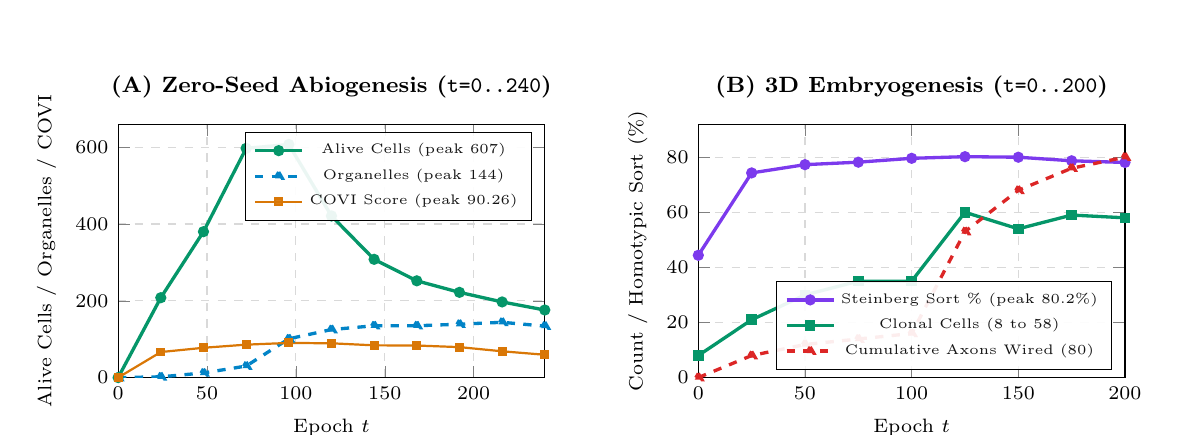
\begin{tikzpicture}
\begin{axis}[
  name=ax1,
  width=7.0cm, height=4.8cm,
  title={\footnotesize\bfseries (A) Zero-Seed Abiogenesis (\texttt{t=0..240})},
  xlabel={Epoch $t$},
  ylabel={Alive Cells / Organelles / COVI},
  xmin=0, xmax=240, ymin=0, ymax=660,
  grid=major, grid style={dashed, gray!30},
  legend pos=north east,
  legend style={font=\tiny, fill=white, fill opacity=0.92},
  label style={font=\scriptsize}, tick label style={font=\scriptsize}
]
  \addplot[color=cmEmerald, very thick, mark=*, mark size=1.4pt] coordinates {
    (0,0) (24,208) (48,380) (72,597) (96,607) (120,421) (144,308) (168,252) (192,222) (216,197) (240,176)
  };
  \addlegendentry{Alive Cells (peak 607)}

  \addplot[color=cmCyan, very thick, dashed, mark=triangle*, mark size=1.5pt] coordinates {
    (0,0) (24,2) (48,12) (72,30) (96,101) (120,125) (144,135) (168,135) (192,139) (216,144) (240,134)
  };
  \addlegendentry{Organelles (peak 144)}

  \addplot[color=cmGold, thick, mark=square*, mark size=1.2pt] coordinates {
    (0,0) (24,66.49) (48,77.61) (72,85.77) (96,90.26) (120,89.29) (144,83.99) (168,83.47) (192,79.34) (216,68.48) (240,59.44)
  };
  \addlegendentry{COVI Score (peak 90.26)}
\end{axis}

\begin{axis}[
  at={(ax1.east)}, anchor=west, xshift=1.95cm,
  width=7.0cm, height=4.8cm,
  title={\footnotesize\bfseries (B) 3D Embryogenesis (\texttt{t=0..200})},
  xlabel={Epoch $t$},
  ylabel={Count / Homotypic Sort (\%)},
  xmin=0, xmax=200, ymin=0, ymax=92,
  grid=major, grid style={dashed, gray!30},
  legend pos=south east,
  legend style={font=\tiny, fill=white, fill opacity=0.92},
  label style={font=\scriptsize}, tick label style={font=\scriptsize}
]
  \addplot[color=cmViolet, very thick, mark=*, mark size=1.4pt] coordinates {
    (0,44.4) (25,74.3) (50,77.3) (75,78.2) (100,79.6) (125,80.2) (150,80.0) (175,78.7) (200,78.1)
  };
  \addlegendentry{Steinberg Sort \% (peak 80.2\%)}

  \addplot[color=cmEmerald, very thick, mark=square*, mark size=1.3pt] coordinates {
    (0,8) (25,21) (50,30) (75,35) (100,35) (125,60) (150,54) (175,59) (200,58)
  };
  \addlegendentry{Clonal Cells (8 to 58)}

  \addplot[color=cmCrimson, very thick, dashed, mark=triangle*, mark size=1.5pt] coordinates {
    (0,0) (25,8) (50,12) (75,14) (100,16) (125,53) (150,68) (175,76) (200,80)
  };
  \addlegendentry{Cumulative Axons Wired (80)}
\end{axis}
\end{tikzpicture}%
}
\caption{Verbatim \texttt{v1.2.1} emergent trajectories with identically $0\,\mathrm{amu}$ / $0\,\mathrm{uq}$ conservation error across every tick: (A)~spontaneous protocell abiogenesis from 0 cells (\code{results/03\_protocell\_abiogenesis.txt}); (B)~zero-blueprint 3D embryogenesis from 8 identical-DNA blastomeres (\code{results/12\_embryogenesis\_grn\_3d.txt}).}
\label{fig:curves}
\end{figure}

\subsection{Endosymbiosis, Xenocellular Solvents, Bioelectricity, Anhydrobiosis, and 13-Vector Ablation}
\begin{itemize}[leftmargin=1.6em, itemsep=1.5pt]
  \item \textbf{Endosymbiosis (\code{results/04}):} Enabling 3D mid-swim endosymbiosis yields 537 captures (181 depth-2 secondary chimeras), 72 EGT events, mean eukaryotic volume $170.21$ vs.\ $53.22$ ablated prokaryotes ($3.20\times$), maximum volume $663.00$ vs.\ $197.00$ ($3.37\times$), high-copy Assembly Index $33.21$ vs.\ $16.00$ ($2.08\times$), and $\mathrm{COVI} = 81.21$ (Stage~5, $\mathrm{MET} = 7/7$) vs.\ $71.08$ (Stage~4, $\mathrm{MET} = 5/7$).
  \item \textbf{Four Planetary Solvents (\code{results/05}):} Table~\ref{tab:solvents} confirms $97.1\%\text{--}99.4\%$ native lipid adaptation and empirical convergence onto the Lean \texttt{T28}--\texttt{T30} c-ring floors. A conservation-exact cross-world transplant ($\mathrm{H}_2\mathrm{O} \to \mathrm{H}_2\mathrm{SO}_4$) triggers 257 acid lyses before rebounding ($73 \to 532$ alive, $\mathrm{COVI} = 77.35$, 0 drift).
  \item \textbf{Bioelectricity \& Anti-Cancer Policing (\code{results/06}):} Gap-junction bioelectricity drives multi-role 3D tissues ($\mathrm{maxT} = 11$ in Track~A vs.\ $0$ in ablated control); Track~B (Feral) records 127 somatic cancer defections, whereas Track~A (Constitutional) suppresses them to $0$ via apoptotic policing.
  \item \textbf{Tardigrade TDP/CAHS Anhydrobiosis (\code{results/07}):} Under 92\% desiccation + 90\% shock lysis (103 pre-shock cells), intact TDP vitrifies 25 tuns $\to$ 25 survive ($12.5\times$ vs.\ 2 in knockout) $\to$ 23 rehydrate and rebound to 97 alive ($\mathrm{COVI} = 76.78$ vs.\ $61.09$).
  \item \textbf{13-Vector Omega Castration Ablation (\code{results/08}):} Zero-restraint feral baseline achieves $\mathrm{COVI} = 82.21$ (0 backlash); 50\% partial restraint triggers the \emph{Escape-Breeding Paradox} across all four channels (79 kill-switch deletions, 486 dormancy spores, 108 HGT smuggles, 1,516 metabolic bypasses; \texttt{DEGRADING 50\%} hormetically overshoots feral baseline to $\mathrm{COVI} = 94.27$, Stage~6); 100\% total restraint extinguishes vitality ($\mathrm{COVI} = 0.00$).
\end{itemize}

\begin{table}[ht]
\centering
\caption{Empirical evolution across four planetary/xenocellular solvents (180 epochs, seed \texttt{5000}, \code{results/05\_xenocellular\_transplants.txt}) confirming convergence onto Lean \texttt{T28}--\texttt{T30} c-ring thresholds.}
\label{tab:solvents}
\footnotesize
\setlength{\tabcolsep}{4pt}
\begin{tabular}{@{} l c c r r r r c @{}}
\toprule
\textbf{Planetary Solvent Regime} & $e_{\mathrm{pmf}}$ & \textbf{Floor $n_H^{\min}$} & \textbf{Alive} & \textbf{Adapted} & \textbf{c-Ring} & \textbf{COVI} & \textbf{Drift} \\
\midrule
Terran Aqueous ($\mathrm{H}_2\mathrm{O}$)        & 10 & $\ge 3$ (\texttt{T28}) & 402 & 98.3\% (395/402) & 3.01 & 84.62 & 0 / 0 \\
Titan Azotosome ($\mathrm{CH}_4/\mathrm{N}_2$)   &  7 & $\ge 4$ (\texttt{T30}) & 295 & 97.6\% (288/295) & 3.95 & 86.96 & 0 / 0 \\
Hydrothermal GDGT Monolayer                      & 10 & $\ge 3$ (\texttt{T28}) & 351 & 99.4\% (349/351) & 4.17 & 77.73 & 0 / 0 \\
Venusian Sulfuric ($\mathrm{H}_2\mathrm{SO}_4$)  & 15 & $\ge 2$ (\texttt{T29}) & 138 & 97.1\% (134/138) & 2.33 & 79.01 & 0 / 0 \\
\bottomrule
\end{tabular}
\end{table}

\subsection{Locked Multi-Arm Paired Statistical Suite (\texorpdfstring{$N = 24$}{N = 24})}
Table~\ref{tab:stats} reports deterministic 10,000-iteration sign-flip permutation tests with Holm--Bonferroni family-wise error-rate (FWER) correction across 24 locked paired seeds (\texttt{5000..5023}, 180 epochs, \code{results/09\_paired\_stats\_n24.txt}). All four pre-registered hypotheses pass decisively ($p_{\mathrm{Holm}} \le 0.00080$).

\begin{table}[ht]
\centering
\caption{Locked paired statistical proof ($N = 24$, seeds \texttt{5000..5023}, 180 epochs; \code{results/09\_paired\_stats\_n24.txt}).}
\label{tab:stats}
\footnotesize
\setlength{\tabcolsep}{4pt}
\begin{tabular}{@{} l r r r c r r @{}}
\toprule
\textbf{Pre-Registered Hypothesis ($N = 24$ Pairs)} & \textbf{Mean A} & \textbf{Mean B} & \textbf{Mean Diff} & \textbf{Wins} & $p_{\mathrm{raw}}$ & $p_{\mathrm{Holm}}$ \\
\midrule
\textbf{H1:} COVI (Feral vs.\ 70\% Castrated)           &  81.768 &  47.194 &  $+34.574$ & \textbf{24/24} & 0.00010 & \textbf{0.00040} \\
\textbf{H2:} Max Cell Vol (Endosymbiosis ON vs.\ OFF)   & 530.292 & 207.708 & $+322.583$ & \textbf{23/24} & 0.00020 & \textbf{0.00080} \\
\textbf{H3:} Bioelectric $\sigma(V_m)$ (ON vs.\ OFF)    &  21.792 &   7.486 &  $+14.306$ & \textbf{24/24} & 0.00010 & \textbf{0.00040} \\
\textbf{H4:} Tardigrade TDP Survival (Intact vs.\ KO)   &  33.125 &   0.542 &  $+32.583$ & \textbf{24/24} & 0.00010 & \textbf{0.00040} \\
\bottomrule
\end{tabular}
\end{table}

% =====================================================================
\section{Scientific Novelty Audit, Honest Epistemic Boundaries, and AI Disclosure}
\label{sec:honesty}
% =====================================================================

\begin{enumerate}[leftmargin=1.6em, itemsep=2pt]
  \item \textbf{Established Science vs.\ Original Contributions:} Non-equilibrium thermodynamics, Chemotons, Mitchell chemiosmosis, Canham--Helfrich bending, Lane's $1/R$ bioenergetic wall, Margulis endosymbiosis, Levin bioelectricity, Boothby TDP bioglass, xenobiological membranes, Fr\"ohlich--Pokorn\'y cytoskeletal modes, Wolpert positional information, Steinberg differential adhesion, and Marder CPG networks belong to their cited original authors~\cite{varela1974,ganti1975,mitchell1961,canham1970,helfrich1973,schnakenberg1976,margulis1967,lane2010,levin2022,boothby2017,frohlich1968,pokorny2004,wolpert1969,steinberg1963,marder2001}. \textbf{No new physical law of nature is claimed}; our GHz microtubule model strictly implements classical ATP-pumped dielectric/acoustic standing-wave modes without endorsing unproven quantum-consciousness hypotheses. Our original contributions are restricted to: (a)~the exact sextic algebraic proof (\texttt{T16}) of the Global Minimax Theorem of Vesicle Division; (b)~the 58-theorem pure Lean~4.35.0 formalization (\texttt{T01}--\texttt{T58}); (c)~the zero-dependency 4-way bit-exact 3D off-lattice C11+AVX2 engine and 60~FPS WebGL2 Observatory; and (d)~reproducible, Holm--Bonferroni-verified emergence across abiogenesis, endosymbiosis, xenocellular solvents, TDP anhydrobiosis, 3D clonal embryogenesis, and restraint-backlash hormesis.
  \item \textbf{Formal-vs-Runtime Boundary \& Coarse-Graining Scope:} The Lean~4 kernel~\cite{demoura2021} certifies exact algebraic and combinatorial invariants of the discrete model equations strictly within \texttt{[propext, Classical.choice, Quot.sound]}. C11 memory layout, SIMD/scalar bit-exactness, \texttt{.cmbin} authentication, stochastic evolutionary trajectories, and statistical inference lie outside the Lean~4 kernel and are tested independently by the 24-gate / 8-mutant executable harness and Ubuntu CI. The engine simulates coarse-grained discrete molecular quanta rather than atomistic wet-lab molecular dynamics, and is not a peer-reviewed journal publication.
  \item \textbf{Transparent AI-Assistance Disclosure:} Substantive AI engineering and formalization assistance (Google DeepMind / Antigravity agent under the author's direction) was used across C11 implementation, Lean~4 proof engineering, falsification testing, and manuscript drafting. AI tools are transparently disclosed and not listed as authors; mathematical and operational claims are independently certified by the Lean~4 kernel, 4-way SHA-256 checksums, GitHub Actions CI, and reproducible falsification tests.
\end{enumerate}

\begin{thebibliography}{37}
\footnotesize
\setlength{\itemsep}{1.2pt}
\setlength{\parskip}{0pt}
\bibitem{varela1974} F.~G. Varela, H.~R. Maturana, and R.~Uribe, ``Autopoiesis: The organization of living systems, its characterization and a model,'' \emph{BioSystems}, vol.~5, no.~4, pp.~187--196, 1974.
\bibitem{ganti1975} T.~G\'anti, ``Organization of chemical reactions into dividing and metabolizing units: the chemotons,'' \emph{BioSystems}, vol.~7, no.~1, pp.~15--21, 1975.
\bibitem{ganti2003} T.~G\'anti, \emph{The Principles of Life}. Oxford University Press, 2003.
\bibitem{mitchell1961} P.~Mitchell, ``Coupling of phosphorylation to electron and hydrogen transfer by a chemi-osmotic type of mechanism,'' \emph{Nature}, vol.~191, pp.~144--148, 1961.
\bibitem{canham1970} P.~B. Canham, ``The minimum energy of bending as a possible explanation of the biconcave shape of the human red blood cell,'' \emph{J. Theor. Biol.}, vol.~26, no.~1, pp.~61--81, 1970.
\bibitem{helfrich1973} W.~Helfrich, ``Elastic properties of lipid bilayers: theory and possible experiments,'' \emph{Z. Naturforsch. C}, vol.~28, pp.~693--703, 1973.
\bibitem{schnakenberg1976} J.~Schnakenberg, ``Network theory of microscopic and macroscopic behavior of master equation systems,'' \emph{Rev. Mod. Phys.}, vol.~48, no.~4, pp.~571--585, 1976.
\bibitem{margulis1967} L.~Sagan [Margulis], ``On the origin of mitosing cells,'' \emph{J. Theor. Biol.}, vol.~14, no.~3, pp.~225--274, 1967.
\bibitem{lane2010} N.~Lane and W.~Martin, ``The energetics of genome complexity,'' \emph{Nature}, vol.~467, pp.~929--934, 2010.
\bibitem{zhu2009} T.~F. Zhu and J.~W. Szostak, ``Coupled growth and division of model protocell membranes,'' \emph{J. Am. Chem. Soc.}, vol.~131, no.~15, pp.~5705--5713, 2009.
\bibitem{svetina2009} S.~Svetina, ``Vesicle budding and the origin of cellular life,'' \emph{ChemPhysChem}, vol.~10, no.~16, pp.~2769--2776, 2009.
\bibitem{hutchison2016} C.~A. Hutchison et~al., ``Design and synthesis of a minimal bacterial genome,'' \emph{Science}, vol.~351, no.~6280, aad6253, 2016.
\bibitem{breuer2019} M.~Breuer et~al., ``Essential metabolism for a minimal cell,'' \emph{eLife}, vol.~8, e36842, 2019.
\bibitem{pelletier2021} J.~F. Pelletier et~al., ``Genetic requirements for cell division in a genomically minimal cell,'' \emph{Cell}, vol.~184, no.~9, pp.~2430--2440, 2021.
\bibitem{levin2022} M.~Levin, ``Technological approach to mind everywhere: An experimentally-grounded framework for understanding diverse bodies and minds,'' \emph{Front. Syst. Neurosci.}, vol.~16, 768201, 2022.
\bibitem{bedau1998} M.~A. Bedau, E.~Snyder, and N.~H. Packard, ``A classification of long-term evolutionary dynamics,'' in \emph{Artificial Life VI}, MIT Press, pp.~189--198, 1998.
\bibitem{taylor2016} T.~Taylor et~al., ``Open-ended evolution: perspectives from the OEE workshop in York,'' \emph{Artificial Life}, vol.~22, no.~3, pp.~408--423, 2016.
\bibitem{sharma2023} A.~Sharma et~al., ``Assembly theory explains and quantifies selection and evolution,'' \emph{Nature}, vol.~622, pp.~321--328, 2023.
\bibitem{stevenson2015} J.~Stevenson, J.~Lunine, and P.~Clancy, ``Membrane alternatives in worlds without oxygen: Creation of an azotosome,'' \emph{Sci. Adv.}, vol.~1, no.~1, e1400067, 2015.
\bibitem{hoshika2019} S.~Hoshika et~al., ``Hachimoji DNA and RNA: A genetic system with eight building blocks,'' \emph{Science}, vol.~363, no.~6429, pp.~884--887, 2019.
\bibitem{seager2023} S.~Seager et~al., ``Stability of nucleic acid bases in concentrated sulfuric acid: Implications for the habitability of Venus' clouds,'' \emph{PNAS}, vol.~120, no.~52, e2220007120, 2023.
\bibitem{seager2024} S.~Seager et~al., ``Year-long stability of nucleic acid bases in concentrated sulfuric acid,'' \emph{Life}, vol.~14, no.~5, 538, 2024.
\bibitem{karr2012} J.~R. Karr et~al., ``A whole-cell computational model predicts phenotype from genotype,'' \emph{Cell}, vol.~150, no.~2, pp.~389--401, 2012.
\bibitem{szigeti2014} B.~Szigeti et~al., ``OpenWorm: an open-science approach to modeling \emph{Caenorhabditis elegans},'' \emph{Front. Comput. Neurosci.}, vol.~8, 137, 2014.
\bibitem{rosen1958} R.~Rosen, ``A relational theory of biological systems,'' \emph{Bull. Math. Biophys.}, vol.~20, pp.~245--260, 1958.
\bibitem{boothby2017} T.~C. Boothby et~al., ``Tardigrades use intrinsically disordered proteins to survive desiccation,'' \emph{Mol. Cell}, vol.~65, no.~6, pp.~975--984, 2017.
\bibitem{hashimoto2016} T.~Hashimoto et~al., ``Extremotolerant tardigrade genome and improved radiotolerance of human cultured cells by tardigrade-unique protein,'' \emph{Nat. Commun.}, vol.~7, 12808, 2016.
\bibitem{thornburg2022} Z.~R. Thornburg et~al., ``Fundamental behaviors emerge from simulations of a living minimal cell,'' \emph{Cell}, vol.~185, no.~2, pp.~345--360, 2022.
\bibitem{caforio2017} A.~Caforio and A.~J.~M. Driessen, ``Archaeal phospholipids: Structural properties and biosynthesis,'' \emph{BBA Mol. Cell Biol. Lipids}, vol.~1862, no.~11, pp.~1325--1339, 2017.
\bibitem{krakauer2020} D.~Krakauer et~al., ``The information theory of individuality,'' \emph{Theory Biosci.}, vol.~139, pp.~209--223, 2020.
\bibitem{frohlich1968} H.~Fr\"ohlich, ``Long-range coherence and energy storage in biological systems,'' \emph{Int. J. Quantum Chem.}, vol.~2, no.~5, pp.~641--649, 1968.
\bibitem{pokorny2004} J.~Pokorn\'y, ``Excitation of vibrations in microtubules in living cells,'' \emph{Bioelectrochemistry}, vol.~63, pp.~321--326, 2004.
\bibitem{sahu2013} S.~Sahu et~al., ``Multi-level memory-switching properties of a single brain microtubule,'' \emph{Biosens. Bioelectron.}, vol.~47, pp.~141--148, 2013.
\bibitem{wolpert1969} L.~Wolpert, ``Positional information and the spatial pattern of cellular differentiation,'' \emph{J. Theor. Biol.}, vol.~25, no.~1, pp.~1--47, 1969.
\bibitem{steinberg1963} M.~S. Steinberg, ``Reconstruction of tissues by dissociated cells,'' \emph{Science}, vol.~141, no.~3579, pp.~401--408, 1963.
\bibitem{marder2001} E.~Marder and D.~Bucher, ``Central pattern generators and the control of rhythmic movements,'' \emph{Curr. Biol.}, vol.~11, no.~23, pp.~R986--R996, 2001.
\bibitem{demoura2021} L.~de~Moura and S.~Ullrich, ``The Lean~4 theorem prover and programming language,'' in \emph{CADE~28}, LNCS~12699, pp.~625--635, 2021.
\end{thebibliography}

\end{document}
